\documentclass[border=5mm]{standalone}
\usepackage{listings}
\usepackage{tikz}
\usetikzlibrary{matrix,backgrounds,decorations.pathreplacing,positioning}
\begin{document}

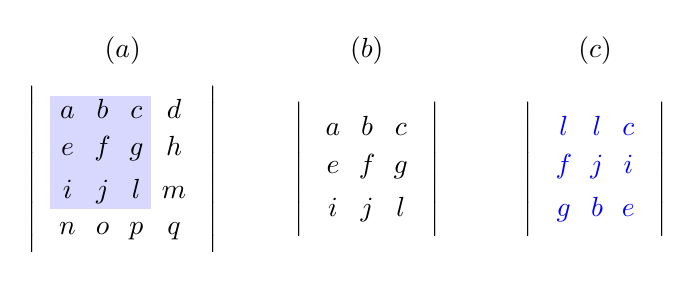
\begin{tikzpicture}[decoration={brace,amplitude=10}]
\matrix(A) [matrix of math nodes,%
            left delimiter  = |,%
            right delimiter = |] at (0,0)
{
 a & b & c & d \\
 e & f & g & h \\ 
 i & j & l & m \\ 
 n &     o & p & q \\
};
\begin{scope}[on background layer]
   \fill[blue!30,opacity=.5] (A-1-1.west|-A-1-3.north) rectangle (A-3-3.south east);
\end{scope}

\matrix(B) [matrix of math nodes,%
            left delimiter  = |,%
            right delimiter = |] at (3.1cm,0)
{
 a & b & c \\
 e & f & g \\ 
 i & j & l \\ 
};


\matrix(C) [matrix of math nodes,%
            left delimiter  = |,%
            right delimiter = |,
            every node/.append style={blue} % <-- added
            ] at (6cm,0cm)
{
 l & l & c \\
 f & j & i \\ 
 g & b & e \\ 
};

%\draw [decorate,thick, red] (A-1-3.north east) -- (A-3-3.south east);
%\draw [thick, red, -latex](A-2-3.east) ++(0.32cm,0) to[out=0,in=180] ([xshift=-.2cm]B.west);
%\draw[->,thick] (B) -- (C) node [pos=0.66,above,font=\footnotesize] {bootstrap};

\node (a) [above=2pt of A] {($a$)};
\node at (a-|B.north) {($b$)};
\node at (a-|C.north) {($c$)};
\end{tikzpicture}
\begin{lstlisting}
Put your code here. 
\end{lstlisting}
\end{document}